%!TEX root=../main.tex
\chapter{Background}
\label{ch:background}
This chapter explains the background for this thesis. Section \ref{sec:mbp} introduces the Mont Blanc Project, the project goals, and its current status, as well as the largest and most significant prototypes. Section \ref{sec:cmb} will present the \gls{cmb} project, the \gls{cmb} system architecture, energy measurement procedures, code correctness and development tools, and finally the planned project development to be made during the Spring of 2016. The chapter finishes with a presentation of related work, presenting other \gls{ojs} as well as relevant crowdsourcing web sites.

\section{The Mont Blanc Project}
\label{sec:mbp}
The \gls{mb} project \cite{MB} started in October 2011. The project received 14 million Euros as initial funding, and the European Commission granted 8 of those millions. The project received an additional funding of 8 million Euros from the European Commission after two years. With a total funding of 22 million Euros, it was estimated that the project would last until September 2016. The project has also been extended as of October 2015, with an extended budget of 7.9 million Euros funded by the European Commission. As mentioned in section \ref{sec:mot}, the long-term goal is to develop an \gls{hpc} architecture with Exascale performance that uses 15 to 30 times less energy than other \gls{hpc} systems. The energy performance metric used is FLOPS/W, motivated by the Green500 list \cite{GREEN500}. The project is split into three phases; the first two coordinated by the Barcelona Supercomputing Center \cite{BSC}, while Bull \cite{BULL} coordinates the third phase.

\subsection{Project Goals and Status}
Both Ramirez \cite{p:MB-PRACE-14} and Mantovani \cite{p:MB-15} summarized the goals of the first two project phases. Mont-Blanc phase 1, valid from 2011 to 2015, had three main objectives. The first was to deploy a prototype scalable to 50 PFLOPS with a total power consumption of 7MW using the available energy efficient embedded technology, which should be competitive with the Green500 leaders of 2014. The second objective was to overcome some limitations found during development and use the gained knowledge in the design of the next generation HPC system. They aimed for an HPC architecture that should be scalable to 200 PFLOPS on 10 MW, which should be competitive with the Top500 leaders of 2017. The third and last objective was to port and optimize Exascale scientific applications capable of exploiting the new generation HPC systems described in objective 2. \\*

The \gls{mb} project phase 2 valid from 2013 including September 2016 has four objectives. The first objective is to supplement the Mont-Blanc prototype, presented below, software stack with software development tools and support ARMv8 \gls{isa}. The second goal is to construct the initial definition of the Exascale architecture, which involved deployment of small ARM-based mini-clusters and evaluation of their suitability in \gls{hpc}. Objective number three is to be up to date with newly released ARM products and evaluate if they are suitable for \gls{hpc} architectures. The last and fourth objective is continued support for the Mont Blanc project. These objectives is also summarized by Follan and Støa \cite{mt:T&S} and on the \gls{mb} project website \cite{MB}.\\*

Mantovani reported the project status in July 2015 \cite{p:MB-15}. Among the tasks finished so far are the deployment of a software stack to support the Mont-Blanc system (see prototype below), porting of new HPC kernels and applications, and design, development, deployment and monitoring of the Mont-Blanc prototype. Amidst the ongoing work is ARM 64 bit exploration, porting new applications for the HPC architecture developed, enhance the programming model (OmpSs \cite{OMPSS}) used and monitor the Mont-Blanc prototype for fault tolerant techniques. \\*

The third phase of the project started in October 2015. The goal is to design a new HPC platform that can improve the performance-energy ratio when executing actual applications. The new design will be developed using a hardware-software co-design \cite{a:MG1997} approach, and will ensure that hardware and system innovations are transformed into HPC application benefits.

\subsection{Prototypes}
Multiple prototypes have been announced, and the specifications of the most significant prototypes are listed below:
\begin{enumerate}
\item \textbf{Tibidabo} \cite{a:MB:Tib}: Tibidabo is the first prototype of the MB project. The prototype is an experimental system and a proof-of-concept HPC system, to show that it is possible to deploy a large scale HPC cluster using ARM processors. The prototype contains compute-boards with NVIDIA Tegra 2 SoC, with dual core ARM Cortex A9 @ 1GHz. The GPUs on the chip did not support the standard programming models OpenCL and CUDA and were therefore not used in the cluster. However, the compute cards can be replaced with up-to-date chips as they become available with updated GPUs that support the two programming models. The prototype consists of 128 nodes each containing a Q7 \footnote{The specific module is taken out of production, but more incormation can be found in \cite{a:MB:Tib}.} module; each module holds a Tegra 2 chip. The prototype achieves 120 MFLOPS/W on High-Performance Linpack (HPL) benchmarks.
\item \textbf{Pedraforca} \cite{p:MB:Pedr}: Pedraforca consist of a combination of ARM processors and NVIDIA GPU’s. One compute node includes a NVIDIA K20 GPU and a Tegra 3 Q7 Module containing 4 ARM Cortex A9 @ 1.3 GHz. The system includes 78 such compute nodes. It is the first large scale HPC system that makes use of ARM-based processors. Even though some factors of the initial technology stack limits the system, the prototype contributes towards the use of ARM-based embedded processors in HPC systems.
\item \textbf{Mont Blanc} \cite{p:MB:MB-prot, p:MB-15}: The latest prototype from the \gls{mb} project. The system contains a rack with a total of 1080 Exynos 5 compute cards, or 2160 ARM Cortex-A15@1.7 GHz CPUs, 1080 ARM Mali T604 GPUs, 4.3 TB of RAM and 17.2 TB of Flash memory. The performance is about 35 TFLOPS and the power consumption is about 24 kW. In November 2014, the Mont Blanc Prototype had an energy efficiency of 1.5 GFLOPS/W. The best Green500 ranking during that time was approximately 5.2 GFLOPS/W.
\end{enumerate}

\section{The Climbing Mont Blanc Prototype}
\label{sec:cmb}
\gls{cmb} is an \gls{oj} focusing on energy efficient programming on ARM based platforms, greatly inspired by the Mont Blanc project. An \gls{oj} is a web application or web based software system which let its users upload programming solutions to defined set of programming problems. Most Online Judges serve problems with varying degrees of difficulty, and can compile and run multiple programming languages (see more in section \ref{sec:related}). The paper "\textit{Climbing Mont Blanc - A Training Site for Energy Efficient Programming on Heterogeneous Multicore Processors}" \cite{a:CMB} and the master thesis of Torbjørn Follan and Simen Støa \cite{mt:T&S} describes the system in great detail. \\

\gls{cmb} is to the best of our knowledge the first \gls{oj} system that focuses on heterogeneous programming and measures energy consumption of submitted programs. The source code is held in a private repository on Bitbucket \cite{BITBUCKET}, that uses \texttt{git} \cite{GIT} as version control. The architecture of \gls{cmb} is shown in Figure \ref{fig:cmb_arch}. As seen in the Figure, the system consists of three main parts; the \textit{frontend}, the \textit{server} and the \textit{backend}. The three parts of the system are explained in detail below. Keep in mind that the below sub-sections presents the prototype \textit{before} any improvements were made to the system. Chapter \ref{ch:improvements} presents, as mentioned, the implementations made in this thesis.

\begin{figure}
  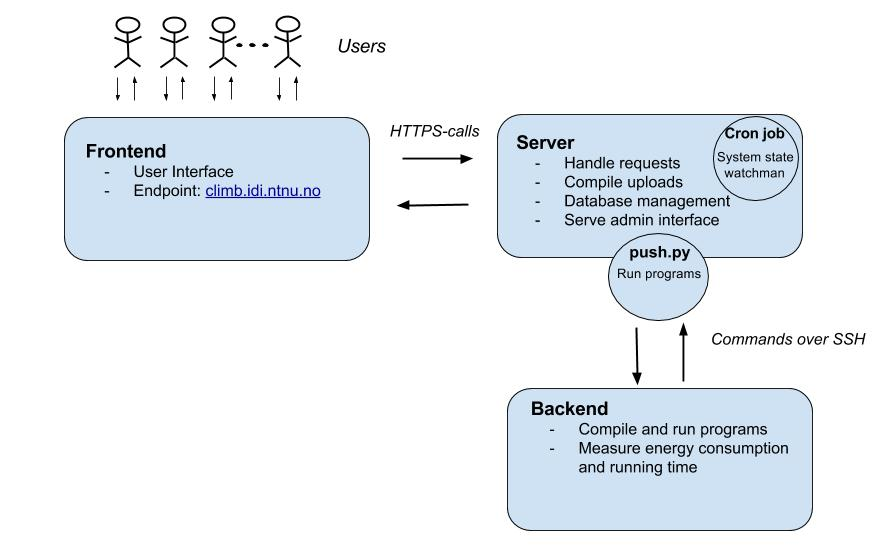
\includegraphics[width=1.0\textwidth]{figs/cmb_arch.jpg}
  \caption[The Climbing Mont Blanc System Architecture]{The Climbing Mont Blanc System Architecture}
  \label{fig:cmb_arch}
\end{figure}

\subsection{Frontend}
\label{subsec:cmb-arch-frontend}
The frontend handles all user based interaction. It is developed in AngularJS \cite{ANGULARJS}, which is a framework developed by Google and is maintained by Google and individual developers. The current frontend uses Angular version 1.3 and Javascript ECMAScript 5th edition. Angular is based upon the \gls{mvc} pattern \cite{b:mvc} and extends HTML with dynamic views with two-way data binding for building single page applications. The result is a smoother user experience, as views updates dynamically with model changes without the need of manually refreshing the web page. The framework also lets the developer define own reusable components, which in most situations make the code base more structured. The view structure and styling are defined in HTML5 and CSS3 respectively. Google Analytics, an advanced monitoring service provided by Google, monitors user interaction at the frontend. Among the things monitored is the number of active users, number of new users and user behavior. \\

\begin{figure}
    \centering
    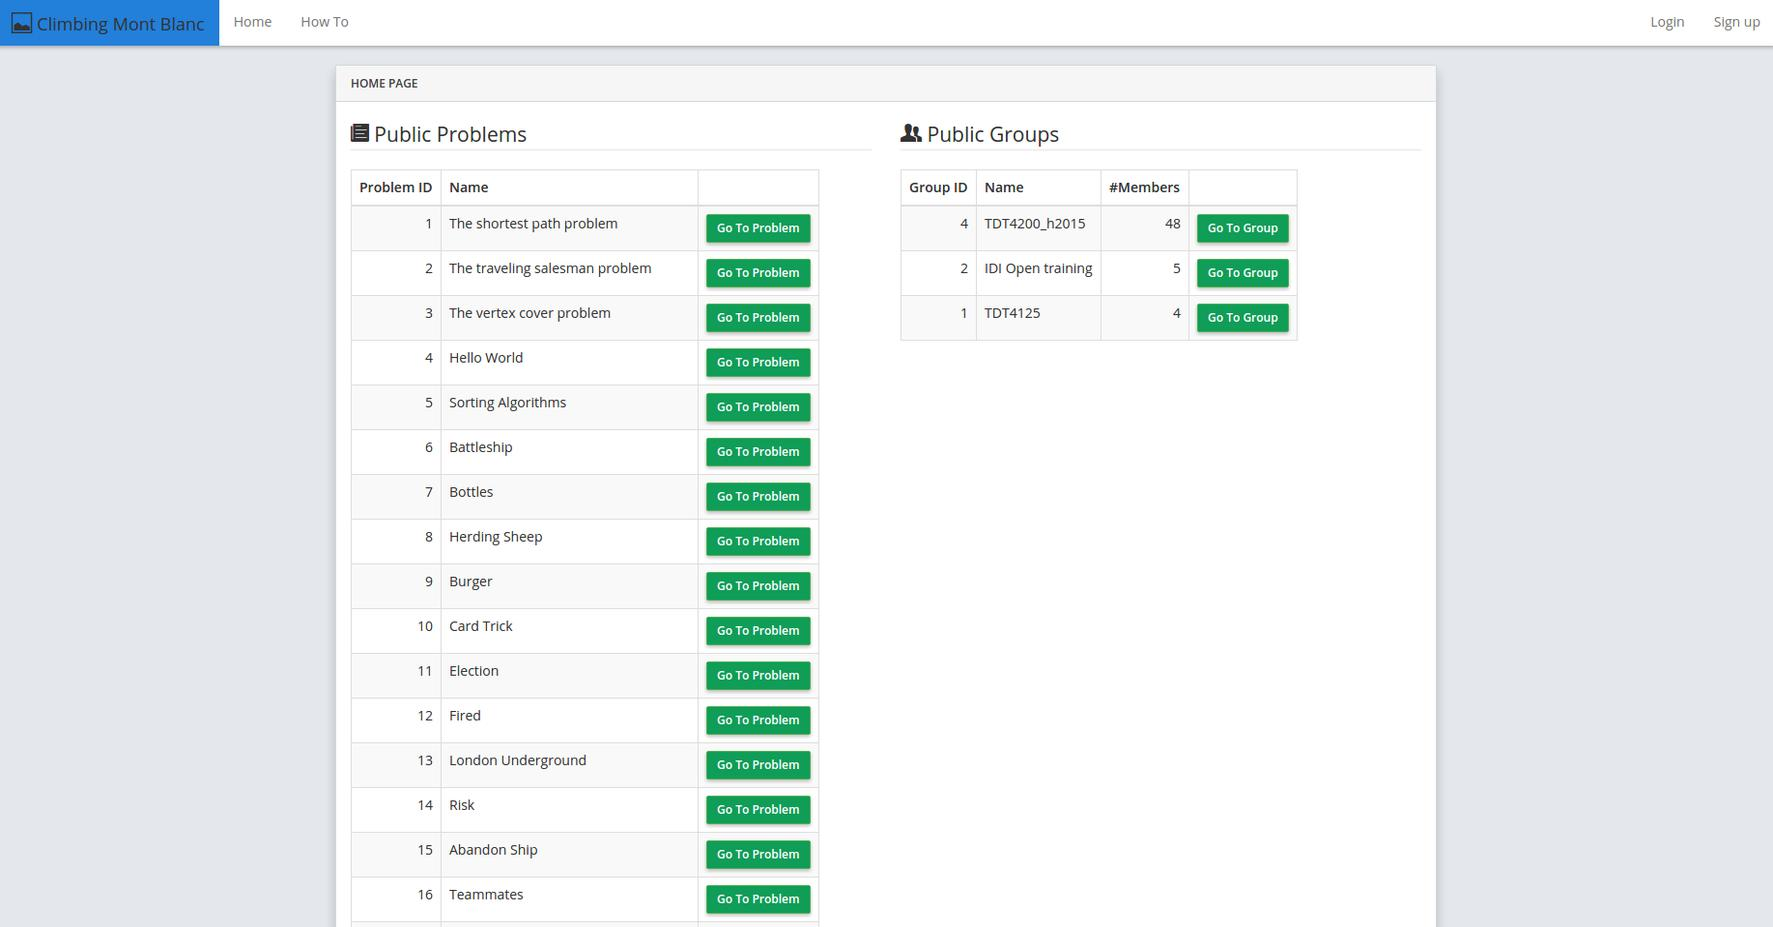
\includegraphics[width=1\textwidth]{figs/front_page.jpg}
    \caption{\gls{cmb} Home Page}
    \label{fig:front-page}
\end{figure}

\begin{figure}
    \centering
    \begin{subfigure}[b]{0.82\textwidth}
        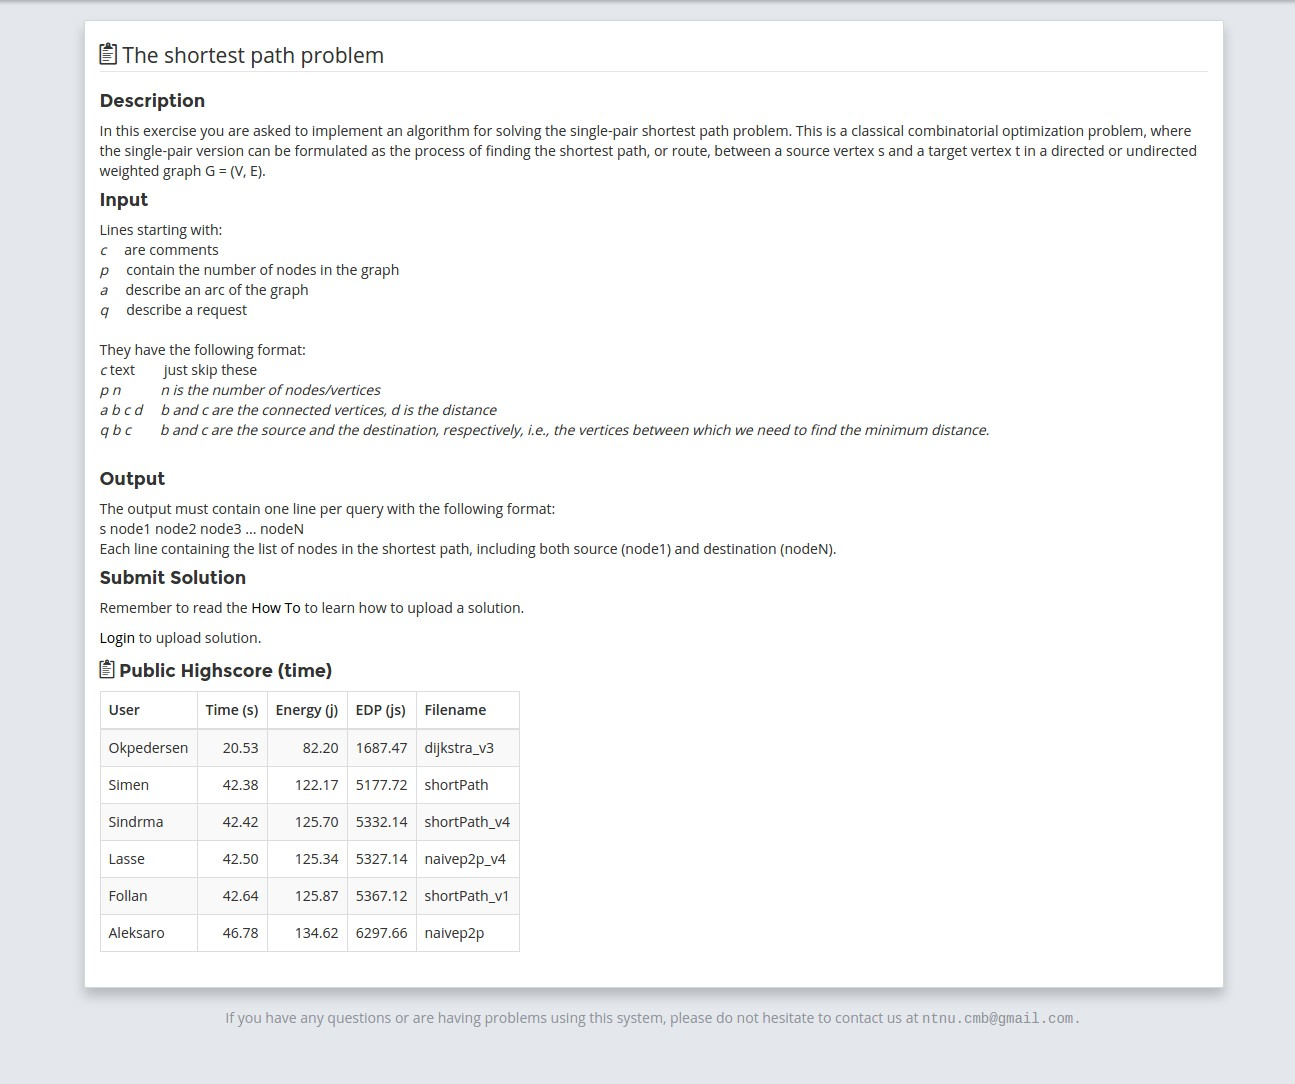
\includegraphics[width=\textwidth]{figs/problem.jpg}
        \caption{Problem View, logged out of \gls{cmb}}
        \label{fig:problem}
    \end{subfigure}
    ~ %add desired spacing between images, e. g. ~, \quad, \qquad, \hfill etc.
    %(or a blank line to force the subfigure onto a new line)
    \begin{subfigure}[b]{0.82\textwidth}
        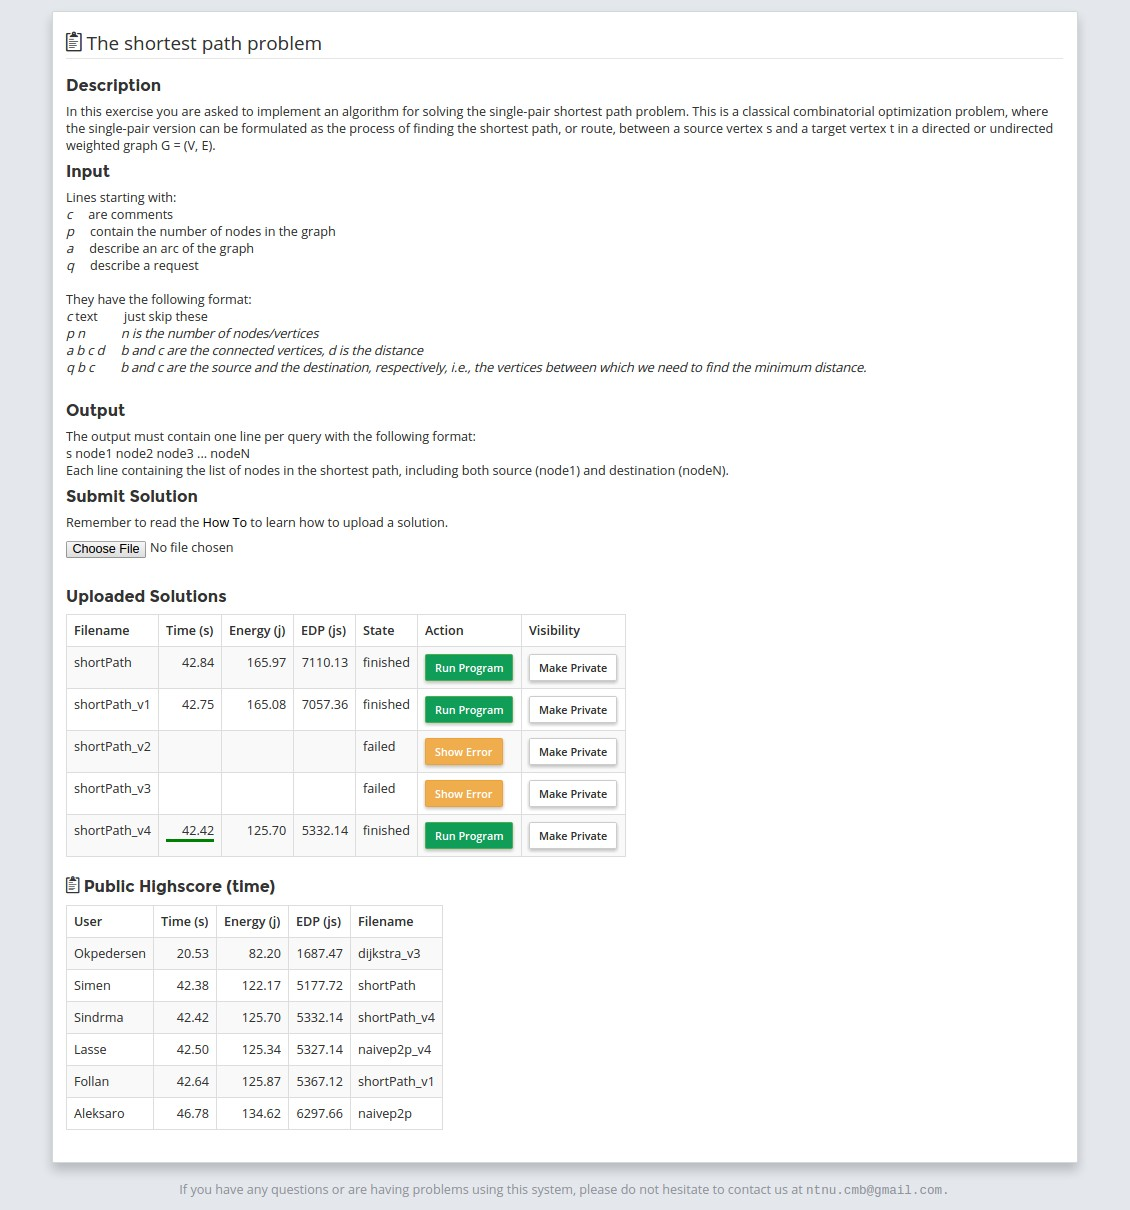
\includegraphics[width=\textwidth]{figs/problem_loggedin.jpg}
        \caption{Problem View, logged into \gls{cmb}}
        \label{fig:problem-loggedin}
    \end{subfigure}
    \caption{\gls{cmb} Problem View States}\label{fig:problem-view}
\end{figure}

The system frontend can be reached at \url{https://climb.idi.ntnu.no} and the front page view is shown in Figure \ref{fig:front-page}. Many actions against the frontend, such as routing to a different view, launches \gls{http} requests to the server that changes models and updates the views dynamically. Angular controllers make these requests to fetch up-to-date data to the frontend models or to update the database with changes made to the models by the user. Routing to a particular problem is an example of dynamic updates of the view, and also displays different views depending on the users state. If the user is not logged in, as shown in Figure \ref{fig:problem}, the view only shows the submitted programs that are \textit{visible}\footnote{A user may change the visibility of their submissions and results through the user interface.}. If the user then logs into the system, as shown in \ref{fig:problem-loggedin}, the problem view changes to make it possible to upload files and view previous submissions. Besides, many actions can be performed in the frontend like routing to a specific problem, login, sign up, create and join groups, manage groups, view the HowTo-page, see public problems and route to a particular problem to solve. The most common action is to upload possible solutions to a problem, which requires a zipped folder containing all source files. \\

\subsection{Server}
\label{subsec:cmb-arch-server}
The server is implemented as an \gls{rest} \gls{api}, as defined in by Roy T. Fielding et.al \cite{a:rtf}. The server is stateless, that is, the user state is stored at the frontend. It is also uniform, meaning that requests sent uses the same data format independent of the technologies used at the server and frontend. The \gls{rest}ful \gls{api} is implemented using Python Flask \cite{FLASK} and the data format used is \gls{json} \cite{JSON}. Our development and production servers also make use of Gunicorn \cite{GUNICORN} to handle simultaneous requests from multiple users. Gunicorn forks off multiple workers upon server startup, each having a private instance of the Flask webserver, and routes incoming requests to the current available workers. If no workers are available, the requests is stalled until a worker becomes idle. \\

Nginx \cite{NGINX} is used as a \textit{reverse proxy} on our development and production server. A reverse proxy serves static files on the fly while requests for dynamic content\footnote{Dynamic content is data that changes during runtime, such as database content.} are forwarded to Gunicorn. SQLite \cite{SQLITE} is used as database with SQLAlchemy \cite{SQLALCHEMY} on top. SQLAlchemy functions as an \gls{orm}, that is, it associates Python classes with database tables and objects of those classes with rows in the tables. SQLAlchemy makes it easy for the programmer to interact with the database, since SQL-statements are abstracted into Python objects and procedures. The underlying database schema is shown in Figure \ref{}.\\

The server runs within a Python \textit{Virtual Environment} \cite{VIRTUALENV} that have all Python required dependencies\footnote{Dependencies is meant by dependencies in between packages (read: code libraries or code \gls{api}s). As an example, SQLAlchemy might require a specific version of Python Flask installed in order to work correctly.} installed. The virtual environment contains only the packages needed by the server, which removes potential dependency errors if the server is to host other Python-based systems in the future. The server is responsible for handling requests from the client, storing useful information in the database and filesystem, and compiling submitted programs. \\

A Python program called \texttt{push.py} runs in the background, regularly checking a \gls{fifo} queue for runnable programs. If a program is ready to run, the script will push the program from the server queue to the backend, and then compile and run it using \gls{ssh}. The result is returned to the server when execution terminates, and the server checks the correctness of the program before reporting the result back to the frontend. Further, the server is responsible for monitoring the state of the system with a background cron job. The cron job runs every 15 minutes, checking if the three system parts Gunicorn, \texttt{push.py} and backend is up and running. The system sends out an automatic e-mail to the system administrators in case of system failure. \\

The server also provides an administrator interface. Admin users have special privileges which grant them access to the admin interface found at \url{http://climb.idi.ntnu.no/admin}. Procedures that modify the database or the server file system are all done through the admin interface. The admins control a lot of the content visible on the frontend, such as programming problems visibility. The most common administrator operation is to add new problems, which requires the admin to add a new problem to the database and upload all files needed to the server. \\

The files needed to make a problem solvable are a input file to be piped into the submitted programs, a file that hold the expected result of an execution and a special file called \texttt{checker.cpp} that checks the correctness of submitted programs. When a program is executed, the input files are given as arguments to the submitted program. When the program is done executing, the checker compares the output of the submitted program against the expected answer files. The program is accepted if the checker program approves the program output. Since the checker is a regular C++-program, it is up to the admin to define what sort of output that should be accepted by the checker. Most of the problems available simply check the difference between output and expected output using the Unix \texttt{diff} program \cite{DIFF}. A special database field called \textit{goodness} can also be added to the problem. The database field is meant for approximation problems to check how ``good'' a solution is. As an example, a solution to the Vertex Cover problem might yield a different cover on each run. The admin making the problem can then define in the checker how good a given cover size is.

\begin{sidewaysfigure}
    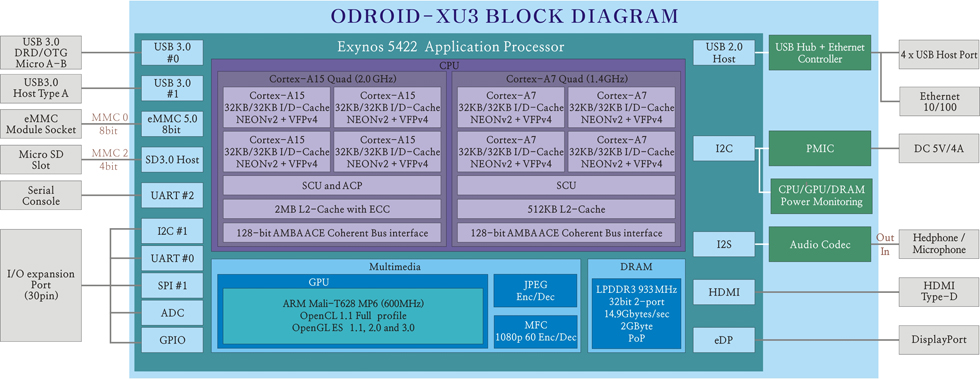
\includegraphics[width=1.0\textwidth]{figs/block-xu3.jpg}
    \caption[Odroid XU3 Block Diagram]{Odroid XU3 Block Diagram (source: Hardkernel Website \cite{XU3-BLOCK})}
    \label{fig:odroid-block}
\end{sidewaysfigure}

\subsection{Backend}
\label{subsec:cmb-arch-backend}
The backend is the executing unit of the CMB system. It is an Odroid XU3 board \cite{XU3} which consists of an Exynos 5 Octa heterogeneous multicore. A block diagram of the board is shown in figure \ref{fig:odroid-block}.  The Odroid board uses a minimal of the external interfaces and components available to get more consistent energy readings; the Ethernet port for internet access, eMMC module or MicroSD card for the \gls{os} image\footnote{The eMMC module loads the \gls{os} image faster than a MicroSD card, and is prefered over a MicroSD card if the module is functional.} and file system, and the board energy monitors. The Exynos 5 Octa consists of four big ARM Cortex A-15 and four small ARM Cortex A-7 cores which share the same \gls{isa}, but have different characteristics when it comes to performance and power consumption. The Exynos chip also has an ARM Mali-T628 GPU with six cores and combined with the two ARM processor types, which makes the Exynos chip a \textit{three-way heterogenous multicore with 14 cores}. \\

The Exynos chip makes use of ARM big.LITTLE technology. The technology enables the \gls{os} to perform Global-Task-Scheduling; to dynamically assign threads to the most appropriate CPU based on the run-time information \cite{ABL}. The board will compile and run the programs pushed to it by the server script \textit{push.py}, measuring time and energy as the program executes. Upon program termination, the board will calculate the program energy consumption and report results back to the server for further processing. The observant reader might view a compilation both at the server and at the board as redundant. Server compilation is done as the server has the capacity to handle multiple users simultaneously, and provides quicker feedback to the user in case of compilation errors. Also, the system lacks a good cross-compiler, and we have not found an appropriate cross-compiler for the server. The backend also needs to compile the submitted program, as the server and backend have different \gls{isa}s. The current CMB backend supports the programming languages C and C++, compiled with gcc-4.9 and g++-4.9 respectively. The compilers have support for both OpenCL v1.1, OpenMP 4.0, NEON and PThreads NTPL 2.19.


\subsection{Energy Measurements}
\label{sec:em-cmb}
The Hardkernel EnergyMonitor program is used to monitor power consumption and is compatible with Odroid XU3 \cite{OEM}. The pipeline in Figure \ref{fig:execution-pipeline} shows the execution pipeline when a program is pushed to the backend. The program is first compiled, and further executed on a small input set to detect potential runtime errors. If there are no runtime errors, the EnergyMonitor program is started and the cache is cleared. Due to energy consumption irregularities found by Follan and Støa \cite{mt:T&S}, clearing the cache is necessary to obtain stable energy readings. After the cache is cleared, the CPU is heated using the UNIX \texttt{stress} \cite{STRESS} command. The CPU runs \texttt{stress} to obtain a fixed start temperature (currently 60 degrees Celsius) before running the program. Starting benchmarks at the same temperature before each run of a benchmark is important to obtain stable energy readings, as pointed out by Cebrian and Natvig \cite{a:JL:T}. The current backend uses the sensors monitoring the temperature of the four big ARM Cortex A15 cores to arrive at the given target temperature of 60 degrees. The program is then executed and, upon program termination, the EnergyMonitor program is ended. Finally, after post processing the program power consumption, the result is reported back to the server. \\

\begin{figure}
  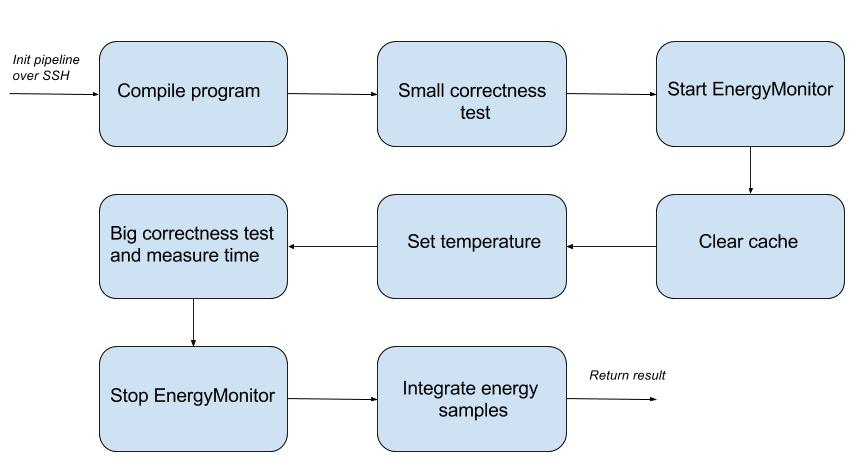
\includegraphics[width=1.0\textwidth]{figs/execution_pipeline.jpg}
  \caption[Backend Execution Pipeline]{Backend Execution Pipeline (adapted from \cite{mt:T&S})}
  \label{fig:execution-pipeline}
\end{figure}

Timestamps are captured right before and right after a program executes to measure execution time. The same timestamps are also used to fetch the power consumption during program execution, by parsing the output of the EnergyMonitor program and select the measurements captured for the big correctness test in the Figure. Upon receiving the results from the backend, the server then calculates the \gls{edp} \cite{a:edp}. This metric is chosen as it emphasizes both energy and performance. Energy is in itself a poor energy efficiency metric since we could simply run a program on a slow and under clocked CPU to obtain low energy consumption. \gls{edp} is defined in Equation \ref{eq:edp}, where \textit{E} is the energy used, \textit{D} is the delay or execution time.

\begin{equation}
  \label{eq:edp}
  EDP = E * D
\end{equation}

The observant reader might have noticed that the Mont Blanc project uses the metric FLOPS/W. This metric may be a useful metric when running the same benchmark, or implementation over and over again to test the energy efficiency of \gls{hpc} and processors architectures. However, \gls{cmb} compares different implementations on the same problems repeatedly, i.e the number of operations may differ from one implementation to the next. Another problem is to determine the number of \textit{useful} instructions, or in other words, instructions that contribute towards solving the problem. For these reasons, \gls{edp} is preferred over FLOPS/W in the \gls{cmb} system and is also the primary energy efficiency metric used in the system.

\begin{table}[b!]
  \centering
  \begin{tabular}{ l|p{2.1cm}|p{2.2cm}|l|l }
    & \textbf{Package Manager} & \raggedright\textbf{Test Framework} & \textbf{Linter} & \textbf{Other} \\ \hline
  \multirow{2}{*}{\textbf{Frontend}} & npm \cite{NPM} & Jasmine \cite{JASMINE} & jshint \cite{JSHINT} & gulp \cite{GULP} \\
                                     & bower \cite{BOWER} & Karma \cite{KARMA} &  &  \\ \hline
  \multirow{1}{*}{\textbf{Server}} & pip \cite{PIP} & nose \cite{NOSE} & flake8 \cite{FLAKE8} & virtualenv \cite{VIRTUALENV}\\
  \end{tabular}
  \caption{\gls{cmb} Code Correctness Tools}
  \label{tab:cct}
\end{table}

\subsection{Code Correctness and Code Deployment}
Unit test frameworks and other tools are used to ensure code correctness in both the frontend and server code. The tools used by the \gls{cmb} system is summarized in table \ref{tab:cct}, and are split into four categories. \textit{Package Managers} are used to install and upgrade dependent code packages and libraries used by the system. The required code packages needed are all listed in special files, one unique file per package manager. Both the frontend and server code makes use of \textit{test frameworks} to develop and run unit- and integration tests and there exist multiple unit tests on both system components. \textit{Linters} are special tools that ensure that language standards are followed, such as semicolons at the end of each line in Javascript or correct indentation in Python files. Other tools include gulp \cite{GULP}, which is a small build system used at the frontend that can execute small user defined tasks, such as running the frontend linter and unit tests or compressing the HTML, CSS, and Javascript files. At the server, virtualenv \cite{VIRTUALENV} is used as a virtual environment as described in sub-section \ref{subsec:cmb-arch-server}. \\

%Rewrite the whole thing
To quickly deploy new features, the system makes use of \textit{Jenkins} \cite{JENKINS} as \gls{ci} server or build server. \gls{ci} is a software engineering practice that automates the testing and deployment of systems. Fowler reports some benefits of CI in his article from 2006; a clone of the production environment (so-called development server) runs tests on the code changes before deployment to production, bugs are discovered and removed easily, and as a whole it makes it possible with rapid integration of new features \cite{a:F:CI}. As briefly mentioned in sub-section \ref{subsec:cmb-arch-server}, the \gls{cmb} system has a development and production server, and these are used to implement \gls{ci} as a practice in the project. The development server is used for manually testing new features in a production-like environment as features are developed. Features that passes the manual testing stage are then deployed to the \gls{cmb} production server. Jenkins can be configured to fit into various system environments, and Figure \ref{fig:server-ci} summarizes its use-case in the \gls{cmb} system. \\

\begin{figure}
  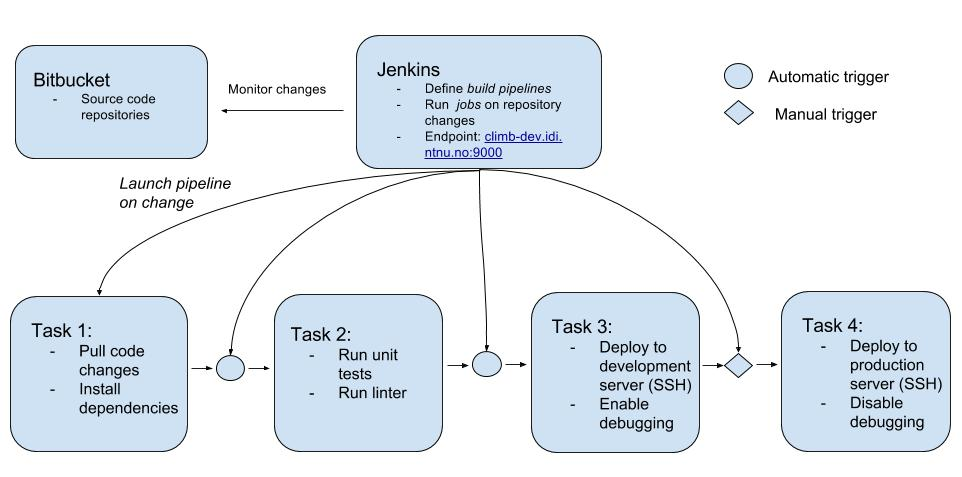
\includegraphics[width=1.0\textwidth]{figs/build_pipeline.jpg}
  \caption[Build Pipeline]{Build Pipeline}
  \label{fig:server-ci}
\end{figure}

The Jenkins \textit{build pipeline} in Figure \ref{fig:server-ci} is defined for both the frontend and server code. Each step in the pipeline is called a \textit{task}, and may have various configurations and use-cases depending on the system environment. The tasks shown in the Figure demonstrates the task configurations used in the \gls{cmb} system. The first task in the pipeline is launched upon code changes on the master-branch in the respective git-repository. The task pulls all the new code changes from git and ensures that installation of package dependencies does not crash the system. If the first task completes without errors, it will automatically trigger the next task which will run all defined unit tests and the linter. As before, if there are no errors, task three is launched which deploys the recent changes to the development server over \gls{ssh} with debugging enabled. If the third task is successful, the code changes should be visible on the development server of \gls{cmb}. \\

Manual acceptance testing and integration tests can be carried out. If the developer(s) are satisfied with the new features, the final and fourth task can be triggered manually. The task deploys the changes to the production server of \gls{cmb}, which also takes care of disabling debugging and compressing the frontend code. Disabling debugging and doing frontend code compression minimizes the number of requests made by the browser and makes the server code execute faster, and it is important to note that this does not affect the functionality of the system. The development server does, as mentioned, have debugging enabled, and uncompressed code to easier find bugs during acceptance testing. Since the difference between the two servers does not sacrifice the functionality of the system, it does not violate the rules set by \gls{ci}.  \\

The \gls{cmb} development server has the a Jenkins server installed and provides a user interface available at \url{http://climb-dev.idi.ntnu.no:9000}.All development should be done locally and then merged with the code on Bitbucket to follow the practice of \gls{ci} correctly. It is considered bad practice to develop code on the development or production server, and the reader should refer to Appendix \ref{apdx:setup} to learn about system setup and local development.

\subsection{Security}

\paragraph*{User Information Security} A number of security measures are taken to make sure that user data are stored and accessed safely. The password is processed by the Python Werkzeug security package \cite{WERKZEUG} upon user creation, to ensure that the password is salted and hashed before being stored in the database. This procedure executes upon both regular and admin user creation. Equal passwords will generate the same hash, but it is very hard for adversaries to reconstruct a password hash. The user sends the password in the login request made to the server \gls{api}, and becomes authenticated if the password hash matches the hash stored in the database. The server then returns a \textit{token}\footnote{A token is some unique string valid for a specific period of time.} which contains enough information to describe uniquely a user-session, and it is sent back in a HTTP response header named \textit{Authorization}. The token is required in some of the requests made to the server \gls{api}, such as uploading and running submissions, and the frontend code takes care of including the header before such requests are made. The token is valid for one hour, which requires a new login after an hour of inactivity. \\

Since the token is stored at the frontend, the server is \textit{stateless} and thereby \gls{rest}ful as mentioned in sub-section \ref{subsec:cmb-arch-server}. To make the transfer of information even more secure, \gls{https} is used to encrypt all the information sent in requests between the server and frontend. \gls{https} use \gls{ssl} to encrypt messages sent to and from the server and is almost impossible to decrypt, which enables safe transfer of passwords and other sensitive data between the server and frontend.

\paragraph*{Uploaded Programs Security} Uploaded program can potentially contain malicious code either in the source files or file names. To restrict the number of possible actions that can be made through the uploaded code, the backend executes the code using a Unix user named \textit{worker} that has minimal \gls{os} permissions on the backend. Also, to remove possible malicious scripts residing in file names, the server again makes use of the Python Werkzeug security package \cite{WERKZEUG} before storing the files in the server file system. It might be worth mentioning that it might be an idea to further extend the system with designated compile servers or threads since unknown errors during compilation might crash the server. Since no such error has occurred, it is listed in Appendix \ref{apdx:backlog} as a possible feature to be added to the system at a later point.

\paragraph*{System Security} The reverse proxy server used at the server is configured to handle \gls{https} requests. As mentioned, the server uses \gls{ssl} when sending and receiving \gls{https} requests. SSL requires an SSL Certificate to work, which is a guarantee that the holder of the certificate provides trustworthy and safe web-content. The most common browsers have a list of trusted third parties issuing certificates, called \gls{cas}, and every certificate issued by one of the \gls{cas} on the list are trusted as safe. Uninett is one example of a \gls{ca} and has created the SSL certificate that is used by the \gls{cmb} system. Since Uninett is a well known \gls{ca}, the \gls{https} requests sent by the system is trusted by most browsers. \\

The \gls{cmb} backend also has \gls{ufw} \cite{UFW} installed. \gls{ufw} which restricts access to the board by requiring every \gls{ssh} request to originate from within the NTNU network. The backend also has Fail2ban  \cite{FAIL2BAN} installed, which restricts the number of authentication attempts made within a certain timeframe. If there are more than three attempts from the same IP-address within the configured timeframe, the IP-address is banned from sending requests for 10 minutes. The server also has \gls{ufw} and Fail2ban installed, but the setup of \gls{ufw} is slightly different. The server \gls{ufw} setup allows all requests made to port 80 and 443 to enable the requests made to \gls{http} and \gls{https} respectively. The setup makes the CMB frontend is accessible from outside the NTNU network. To keep up to date with security updates \texttt{unattended-updates} \cite{UNATTENDED} is enabled on the production server, which installs security updates if needed. The check for security updates are made every night at 02:00, and an automatic restart of the system is done if the update requires it.


\subsection{Other Related CMB Projects}
\label{subsec:related-proj}
\begin{figure}[ct!]
  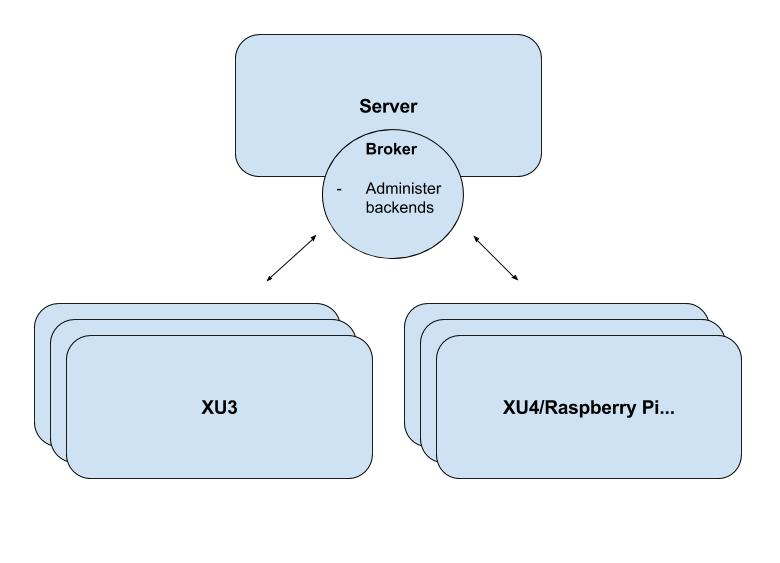
\includegraphics[width=1.0\textwidth]{figs/cmb_scale_arch.jpg}
  \caption[Scalable \gls{cmb} Architecture]{Scalable \gls{cmb} Architecture}
  \label{fig:cmb-scale-arch}
\end{figure}

\subsubsection{System Scalability}
Previous user testing has shown that the system is bottlenecked by the number of executing units. The bottleneck was noticed during the Autumn of 2015 when students had to use the system as part of mandatory exercises in the course TDT4200 Parallel Computing \cite{TDT4200}. The Specialization project report delivered in December 2015 presented feedback given by the TDT4200 students, and some students pointed out that submissions often stalled for several minutes in the run queue with little feedback on progress. Even though students were advised to start exercises early and submit to the system long before exercises were due, the system should still handle a higher load of users duringthe last few hours before the exercises' deadline. Further, if the system is to be used in programming competitions like \gls{icpc} \cite{ICPC} or IDIOpen \cite{IDIOPEN} as well, it needs to handle multiple concurrent submissions without stalling them in the queue for to long. \\

The observations motivated the extension with several execution backends like depicted in Figure \ref{fig:cmb-scale-arch}. Christian Chavez has been assigned the thesis on \gls{cmb} scalability, which should extend the system with more Odroid XU3 boards. The idea is to have multiple backends at the \gls{cmb} production server to handle multiple submissions at the same time, as described in the CMB paper by Natvig et.al \cite{a:CMB}. A control mechanism needs to be implemented, to administer the incoming requests and possible run queue race conditions. This mechanism is called a \textit{broker} in the Figure. Have in mind that the Figure describes the concept of scaling the system with multiple boards, and there are several possible ways to implement the suggested broker. \\

Follan and Støa suggested that one could simply add more push scripts, one script for each connected backend \cite{mt:T&S}. While this solves the problem of extending the system with more boards, the push script has proven to fail and terminate due to some erroneous output from the backend. Finding errors and bugs in bash scripts executed over \gls{ssh} in Python has proven to be difficult to debug, which has driven the project team to look for other solutions than simply extending with more push scripts. The Specialization project report proposed the use of \textit{task queues}, which are mechanisms to distribute work among threads or machines. However, it might impose unnecessary complexity to the system.  \\

The thesis will also describe how the broker can be used to allow different backends other than the currently used Odroid XU3 board. Figure \ref{fig:cmb-scale-arch} also shows n illustration of the architecture if extended with different backends. Allowing various types of boards on the system enables further exciting research on energy efficient programming, and may provide \gls{cmb} users with the possibility of comparing the energy efficiency of benchmarks on multiple architectures in a quick manner.

\section{Related Work}
\label{sec:related}
Sub-section \ref{subsec:oj&c} will present related \gls{ojs} which might inspire the future development of the \gls{cmb} system. The presented work is inspired by the \gls{ojs} presented in the master thesis of Follan and Støa and further extended with interesting \gls{ojs} as well as the \gls{ojs} mentioned in the Specialization project. There exists many \gls{ojs} sites which have a wast amount of users and submissions, but as mentioned, we are not aware of any other \gls{oj} focusing on energy efficient programming. Instead, we present popular \gls{ojs} and their features, which might have an effect on the future development of \gls{cmb}. Further, we also present the most popular crowdsourcing sites as these have some relevance to the project. Table \ref{tab:definitions} lists the definitions of an \gls{oj} (briefly mentioned in section \ref{sec:cmb}) and crowdsourcing. Since crowdsourcing is a broad term we will further restrict the definition: \textit{Crowdsourcing is the action of outsourcing programming tasks and problems to a large group of programmers in the form of an open call}. The definitions are valid throughout the thesis. \\

%The most relevant work we have found within energy efficient programming is the Green Coding contest \cite{GREENCODING} hosted in 2014. However, we have not been successful in finding results from this competition and it has only been hosted once. Instead, we present some of the most relevant work within Energy-Aware programming and software in sub section \ref{subsec:eap}, focusing on work which might effect the energy efficiency measurements and software we have developed to the Odroid XU3.

\begin{table}[t!]
    \centering
    \begin{tabular}{ | l | p{7cm} | }
    \hline
    \multicolumn{2}{ | c | }{\textbf{Definitions}} \\
    \hline
    Online Judge & ``An online based computer system, providing programming problem descriptions and data sets to automatically judge wether a particular solution solves a given problem.'' Inspired by definition found in \cite{a:Kurnia2001}  \\ \hline
    Crowdsourcing & ``The act of taking a job traditionally performed by a designated agent and outsourcing it to an undefined, generally large group of people in the form of an open call.'' \cite{CROWDSOURCING}. \\ \hline
    \end{tabular}
    \caption{Defining \gls{ojs} and Crowdsourcing}
    \label{tab:definitions}
\end{table}

\subsection{Online Judges and Crowdsourcing}
\label{subsec:oj&c}
%Torbjørn Follan and Simen Støa mentioned several of the most popular \gls{ojs} in their Master Thesis \cite{mt:T&S}. The In-Depth study delivered in December 2015 summarized the \gls{ojs} mentioned by Follan and Støa, and further explored trending \gls{ojs} not previously presented. This sub-section will present the \gls{ojs} both presented by Follan and Støa and in the In-Depth study, focusing on unique features and aspects that may inspire the future development of the \gls{cmb} \gls{oj}. The In-Depth study also mentioned the most popular Crowdsourcing websites, and the crowdsourcing sites mentioned in that work will also be briefly introduced in this sub-section. Table \ref{tab:definitions} presents the definitions of an \gls{oj} (mentioned in section \ref{sec:cmb}) and Crowdsourcing, which are valid throughout the thesis. The definition of crowdsourcing is broad, and in this thesis it is further restricted: Crowdsourcing is the action of outsourcing programming tasks and problems to a large group of programmers in the form of an open call. As mentioned earlier, we are not aware of any other \gls{ojs} which focuses on energy efficient programming. The Green Coding contest \cite{GREENCODING} hosted in 2014 is the only work we have found related to energy efficient programming. This sub-section summarizes the \gls{ojs} that is either very popular or has unique factors compared to other \gls{ojs}, and in addition present the most popular crowdsourcing sites within information technology relevant for the CMB project.

\paragraph*{Kattis} \hfill \\
The first version of Kattis was developed in 2005 at KTH in Stockholm \cite{a:Enstrom2011}. The judge was first used for assessing programming exercises in various courses at the university. Since the first version, the Judge has developed into a sophisticated and well known \gls{oj} and is widely used in the Nordic countries, perhaps because of its usage in the programming contests \gls{icpc} \cite{ICPC} and IDIOpen \cite{IDIOPEN}. The judge supports 13 programming languages and offers a broad range of programming problems to solve with varying difficulty. The judge is offered to the public through a website, but it is also offered as a simple \gls{cli}.\footnote{The Kattis \gls{cli} can be found at github: \url{https://github.com/Kattis/kattis-cli}.} \\

Kattis also offers services for firms and universities alongside hosting an public \gls{oj}. Professors can register courses and automatically grade programming exercises, such that students easily can get feedback and track their exercise scores. The service also offers plagiarism checks of submitted code and analytics of the registered courses. Companies can register to challenge potential job candidates with a set of programming problems before interviewing them, and offer crosschecking of submitted code to filter out cheaters. The universities can choose either a free subscription with a limited number of registered courses and teachers, or a premium subscription with an unlimited number of teachers and courses with a cost of 15\$ per student, per course. Companies have three different paid subscriptions to choose from, which offers either a few, medium or large number of interviewers and problems depending on the chosen subscription.

\paragraph*{UVa Online Judge} \hfill \\
The first version of UVa Online Judge \cite{UVA} was developed by former student Ciriaco García de Celis in 1995 \cite{a:Revilla2008}. The judge was first built as a series of bash scripts, but the scripts were later replaced by a team of students to make the judge able to handle the increasing amount of submissions and to ready the system to be used in programming competitions. Today the UVa Online Judge is very popular, with over 1,8 million submissions registered in 2015 and over 100,000 users. The judge also offers over 4,300 programming problems solvable in 6 different programming languages.

\paragraph*{PKU JudgeOnline} \hfill \\
PKU JudgeOnline \cite{PKU} released in 2003 and is one of the \gls{ojs} with the highest number of submissions. At its peak in 2010, the judge had over 1.768 million submissions, but the number of submissions has decreased in recent years measuring almost 1,3 submissions in 2015. The \gls{oj} provides mostly the same features as other \gls{ojs}, like viewing statistics, submitting code to problems, and hosting online contests.

\paragraph*{URI Online Judge} \hfill \\
The URI Online Judge is served through a website which was first presented in July 2012 \cite{a:Bez2013}. The \gls{oj} aims to support both teaching student about programming and professors aiding them to manage courses and exercises. A total of eight problem categories is offered, training students in various topics in programming. Bez et.al also mentions a couple of features implemented. One feature lets the user send in the input test cases to a problem, in which the online judge responds with the correct expected output. Another lets the user view the code directly in the browser during compilation errors, with highlighted code lines on those lines containing errors \cite{a:Bez2013}.

\paragraph*{HackerRank} \hfill \\
HackerRank \cite{HACKERRANK} has over 800,000 developers registered and over 800 public problems and challenges. The project was started in 2008 by Vivek Ravisankar and Hari Karunanidhi. The founders felt like they spent too much time on engineering interviews and less time creating great solutions, and they also had a hard time finding good programmers through the traditional interview process. The \gls{oj} supports over 35 programming languages and offers a clean design in their interface, with features such as online code editing. HackerRank does also have an extensive work section with more than 1,000 companies registered. The companies interested in filling a particular position can create a basic free profile to interview candidates, create or add problems, and watch the candidate code in real-time. One can also request a premium subscription, which has even more advanced features like detecting code plagiarism. It does also have a section for schools that want to create online programming assignments similar other judges providing the same feature.

\paragraph*{HackerEarth} \hfill \\
HackerEarth \cite{HACKEREARTH} has over 14.4 million submissions, 3,146 practice problems, and 232 in-depth tutorials. The HackerEarth team has one goal: make technical recruitment straightforward and efficient. The judge offers much of the same features as HackerRank and the other \gls{ojs} mentioned above but has some unique features as well. They provide a \gls{rest}ful \gls{api} documentation, which can be used to integrate the \gls{oj} with other software systems. The HackerEarth team has also developed a chrome extension to notify their users about upcoming programming competitions and events. The judge also hosts programming competitions, provide practice problems, provide a similar extensive work section as HackerRank, and provide multiple technical and non-technical blogs. HackerEarth can also be seen as a partial crowdsourcing site, with its numerous challenges and hackathons provided by firms on the HackerEarth website.

\paragraph*{LeetCode} \hfill \\
LeetCode \cite{LEETCODE} has about 52,000 users registered. Their goal is to prepare coders for technical IT interviews, and offer much the same features as the other \gls{ojs} above. However, they have a unique feature which is in-depth articles per problem. Each article goes into depth about the theory required to solve the given problem, and the \gls{oj} also enables its users to discuss the articles with other users through their online forum.

\paragraph*{Other popular \gls{ojs}} \hfill \\
There are three more Online Judges that is worth mentioning briefly. These are Timus Online Judge \cite{TIMUS}, A2 Online Judge \cite{A2OJ}, CodeChef \cite{CODECHEF}, and Sphere online judge \cite{SPHERE}. These \gls{ojs} offer features similar to those already presented, so they are not explained in great detail. More information about them can be found on their websites.

\paragraph*{TopCoder} \hfill \\
The crowdsourcing site that seems to be the most popular is TopCoder \cite{TOPCODER}. The site got more than 895,000 members and is used by companies like Amazon, Facebook, IBM, and Microsoft for crowdsourcing real world problems to solve. The best solutions to a problem often get awarded with a money prize.

\paragraph*{RecSys Challenge} \hfill \\
The RecSys Challenge \cite{RECSYS} is a crowdsourcing competition that has been hosted every year since 2010. The competition aims to solve different challenges within recommender systems, where the top three winners receive a money prize and an opportunity to present their solution at the RecSys Conference. Many students at NTNU compete in this competition as a part of their master thesis.

%\subsection{Energy-Aware Programming and Software}
%\label{subsec:eap}

%Simon Holmbacka++ for accurate energy readings and
% fill in with more if discovered
% spørre Lasse om tips her, trenger flere kilder og helst artikler
